\section{Question 3} 
\subsection{PCA-LDA}
\subsubsection{Accuracy}

\begin{figure}[h]
	\centering
	%\fbox{\rule{0pt}{2in} \rule{0.9\linewidth}{0pt}}
	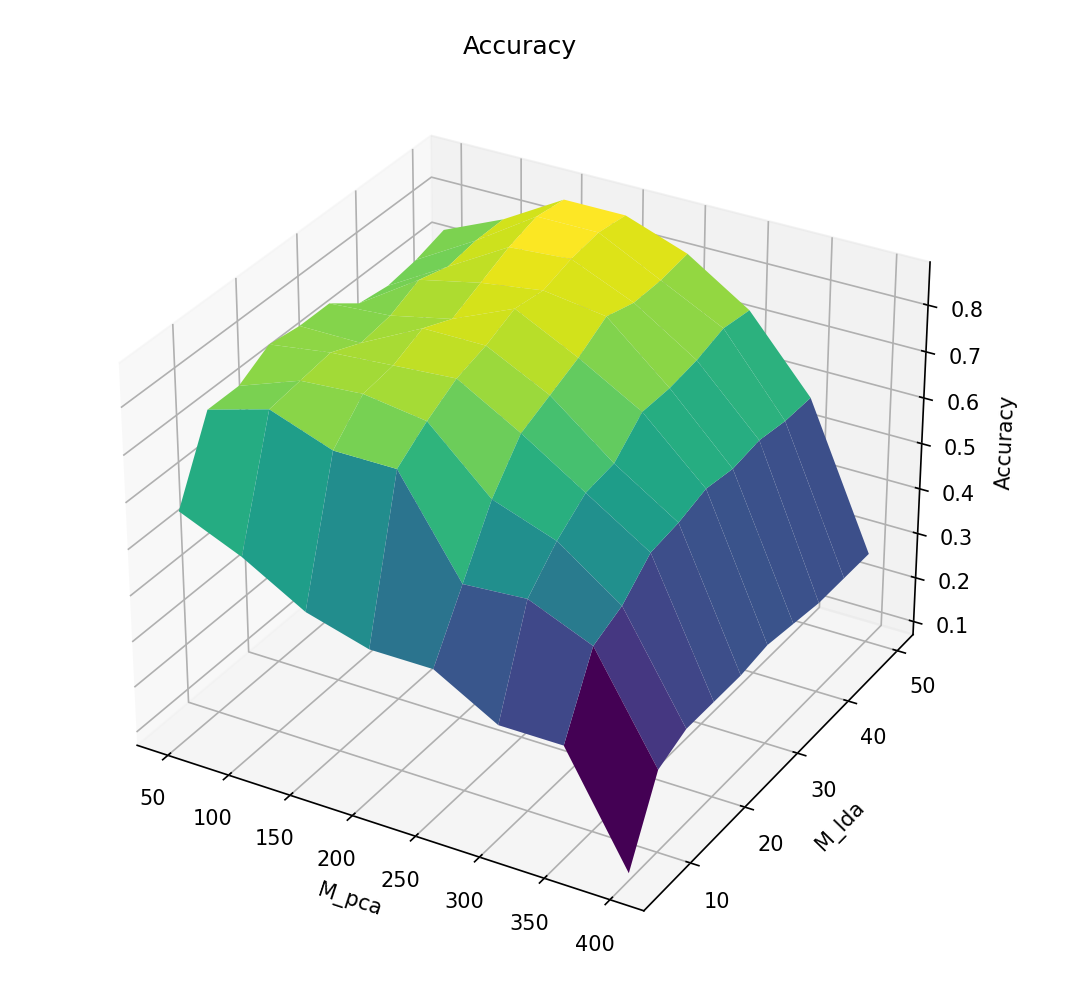
\includegraphics[width=0.8\linewidth]{Ressources/Q3_accuracy1.png}
	
	\caption{Accuracy}
	\label{fig:Q3_accuracy}
\end{figure}

Figure~\ref{fig:Q3_accuracy} shows the influence of M\_pca and M\_lda on accuracy.

For M\_pca, as M\_pca increases, the accuracy generally improves, particularly in the range of lower M\_lda values. But, when M\_pca is too large, overfitting occurs, which negatively impacts the accuracy. This happens because using a large number of PCA components captures more detailed patterns in the data, including noise.

For M\_lda, similarly, an increase in M\_lda initially leads to a moderate improvement in accuracy, but the effect slightly declines at higher values of M\_pca.

The highest accuracy appears to occur when both M\_pca and M\_lda are at optimal values, indicating a balanced approach. However, as either M\_pca or M\_lda gets too high, the accuracy may decrease, potentially due to overfitting or noise in the model.
%-------------------------------------------------------------------------
\subsubsection{Ranks of the scatter matrices}

For the between-class scatter matrix, the rank of Sb is 51, which indicates there are 52 classes in the dataset (since $Rank(Sb)\leq C-1$). This rank reflects the number of linearly independent directions along which the class means differ. In this case, with 51 independent directions, LDA can theoretically create up to 51 discriminative components for optimal class separability.

For the within-class scatter matrix, the rank of Sw is 364, which suggests that there are 364 linearly independent directions in the data that capture the variations within each class. This variability could come from different expressions, lighting conditions, slight head movements, etc.

For the total scatter matrix, the rank of St is 415, since St = Sb + Sw, the rank of St represents the total variability across all samples, both within and between classes. This implies that there is very little redundancy in the overall data structure and that the data spans almost the entire feature space. And PCA can reduce the data from 2576 dimensions down to 415 dimensions without losing information.

%-------------------------------------------------------------------------
\subsubsection{Confusion matrix and Cases}

\begin{figure}[h]
	\centering
	%\fbox{\rule{0pt}{2in} \rule{0.9\linewidth}{0pt}}
	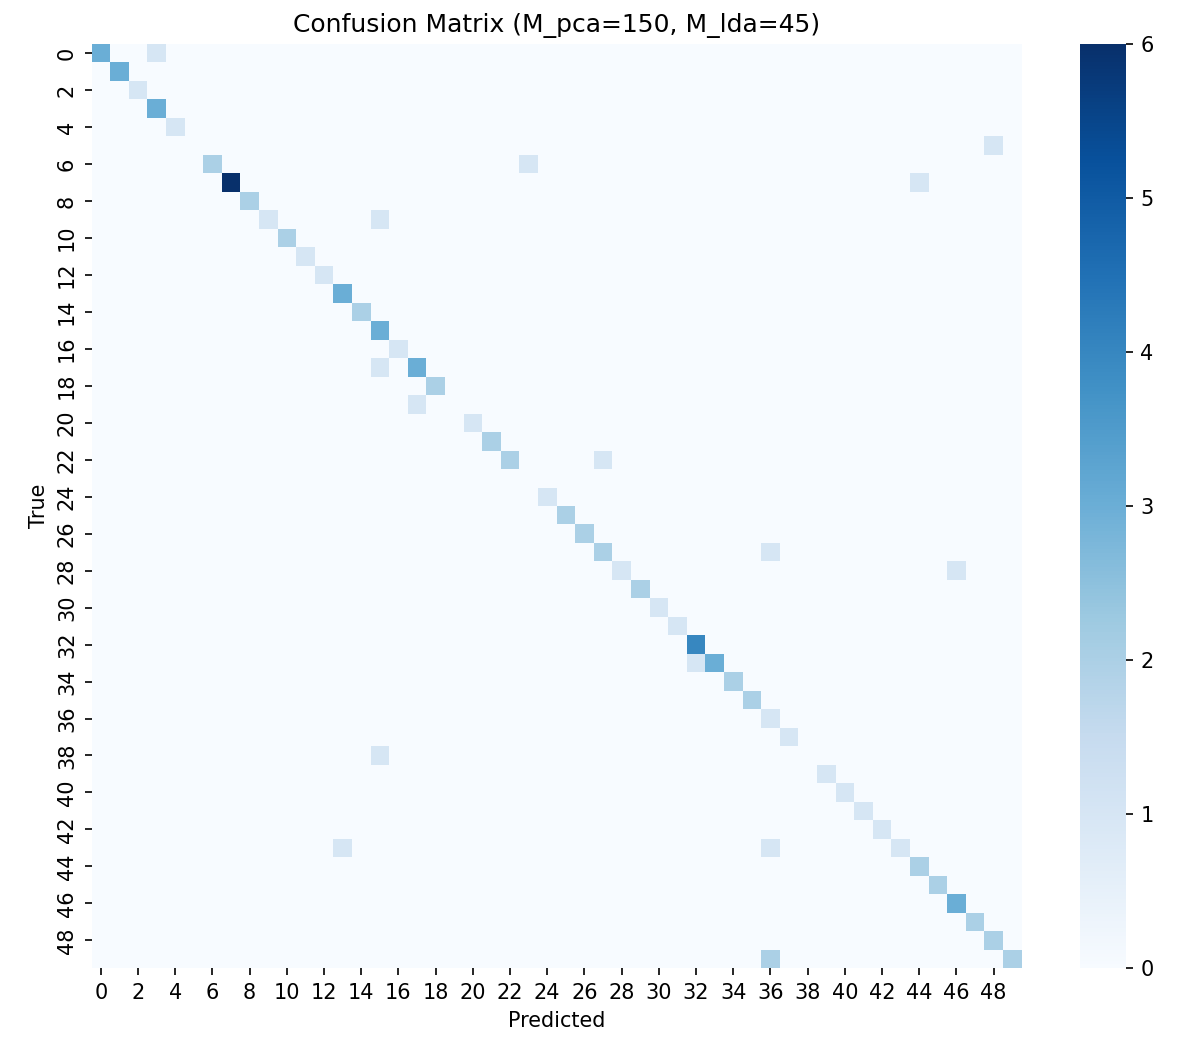
\includegraphics[width=0.8\linewidth]{Ressources/Q3_cm.png}
	
	\caption{Confusion Matrix}
	\label{fig:Q3_cm}
\end{figure}

Figure~\ref{fig:Q3_cm} shows the model is generally effective in distinguishing most classes, as seen by the concentrated diagonal line of correct predictions. And Figure~\ref{fig:Q3_cases} shows success and failure cases.

\begin{figure}[h]
	\centering
	%\fbox{\rule{0pt}{2in} \rule{0.9\linewidth}{0pt}}
	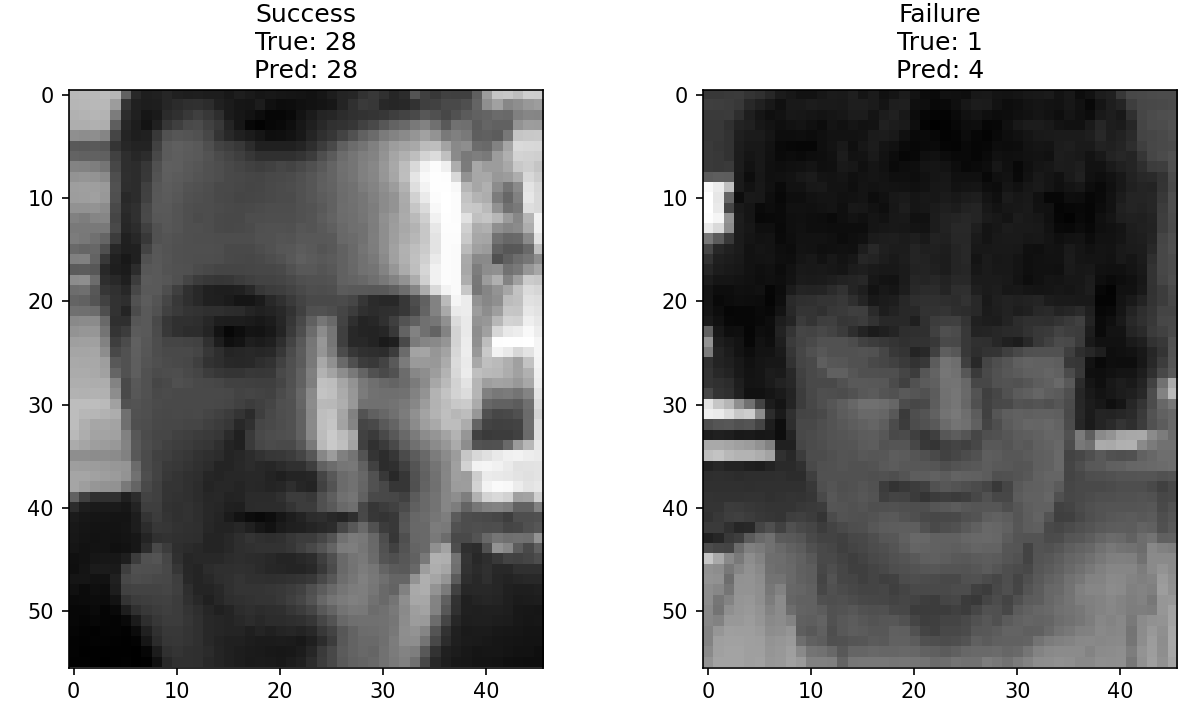
\includegraphics[width=0.8\linewidth]{Ressources/Q3_cases.png}
	
	\caption{Success and failure cases}
	\label{fig:Q3_cases}
\end{figure}

%-------------------------------------------------------------------------
\subsubsection{Comparison to Q1}

%-------------------------------------------------------------------------
\subsection{PCA-LDA Ensemble}

\subsubsection{Randomisation}
\begin{figure}[h]
	\centering
	%\fbox{\rule{0pt}{2in} \rule{0.9\linewidth}{0pt}}
	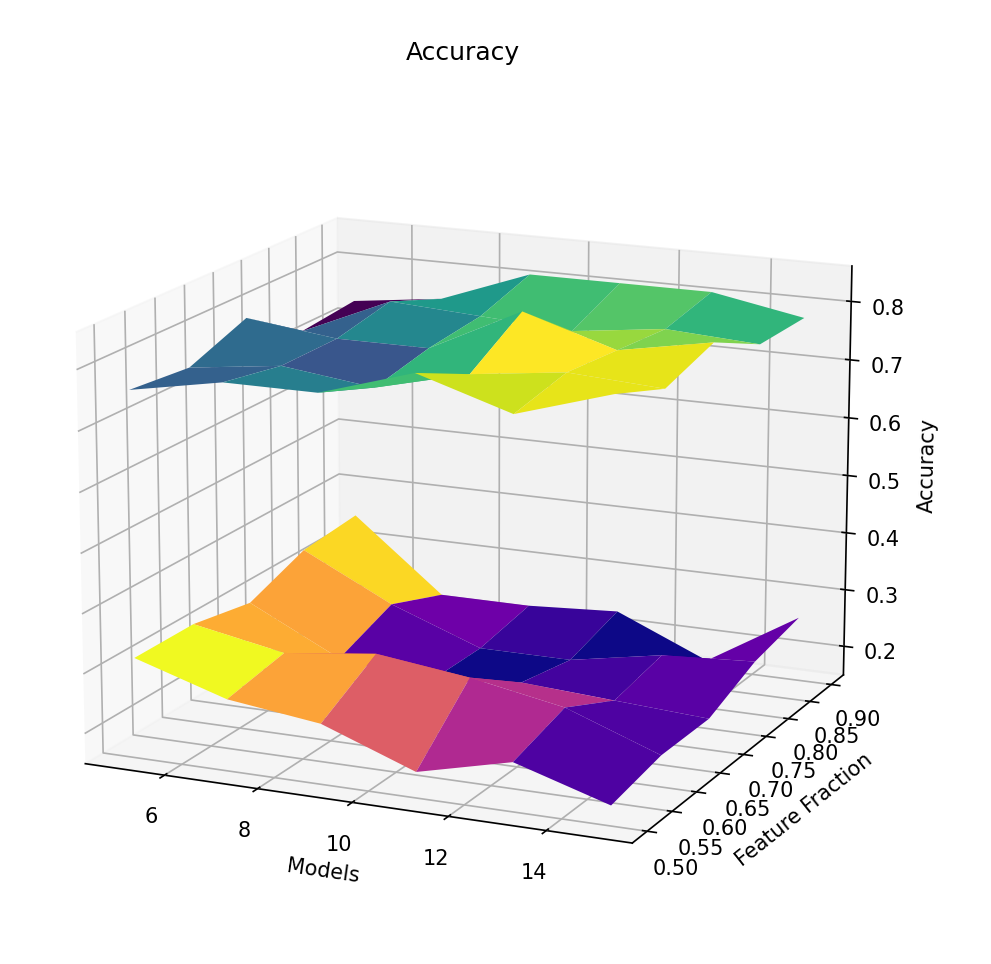
\includegraphics[width=0.8\linewidth]{Ressources/Q3_acc_f.png}
	
	\caption{Accuracy with randomisation in feature space}
	\label{fig:Q3_acc_f}
\end{figure}
Increasing the number of base models generally improves the ensemble’s robustness and stability, as it reduces the variance and makes the model less sensitive to the performance of any individual base model.